\documentclass[10pt, oneside]{article} 
\usepackage{amsmath, amsthm, amssymb, calrsfs, wasysym, verbatim, bbm, color, graphics, graphicx, geometry}
\usepackage[most]{tcolorbox}
\usepackage{xcolor}
\usepackage{framed}
\colorlet{shadecolor}{blue!15}
\graphicspath{ {./} }

\geometry{tmargin=.75in, bmargin=.75in, lmargin=.75in, rmargin = .75in}  

\newcommand{\R}{\mathbb{R}}
\newcommand{\C}{\mathbb{C}}
\newcommand{\Z}{\mathbb{Z}}
\newcommand{\N}{\mathbb{N}}
\newcommand{\Q}{\mathbb{Q}}
\newcommand{\Cdot}{\boldsymbol{\cdot}}

\newtheorem{thm}{Theorem}
\newtheorem{defn}{Definition}
\newtheorem{conv}{Convention}
\newtheorem{rem}{Remark}
\newtheorem{lem}{Lemma}
\newtheorem{cor}{Corollary}
\newtheorem{exa}{Example}


\title{Clase \# 1: Propiedades de los fluidos [MF100]}
\author{\textbf{Luis Alejandro Morales}\\ \vspace{0.4cm} Profesor Asistente \\ Universidad Nacional de Colombia-Bogot\'a\\Facultad de Ingenier\'ia \\ Departamento de Ingenieria Civil y Agr\'icola}
\date{Periodo 2022-II}

\begin{document}

\maketitle
\tableofcontents

\vspace{.25in}

\section{Introduccion}
\begin{defn}
La mecanica de fluidos es la ciencia que hace parte de la mecanica clasica la cual estudia los fluidos estaticos o en movimiento y su interaccion con otros objetos o fluidos.
\end{defn}
La mecanica de fluidos puede ser dividida en differentes categorias:
\begin{itemize}
\item \textbf{Hidrodinamica}: La cual estudia fluidos en moviento que pueden ser considerados inconpresibles e.g. agua and gases a bajas velocidades.
\item \textbf{Hidraulica}: Estudia el movimiento de liquidos en tuverias y canales abiertos (e.g. Rios).
\item \textbf{Dinamica de gases}: Estudia el flujo de fluidos sometidos a cambios importantes de la densidad, e.g. flujo de gases a alta velocidad.
\item \textbf{Aerodinamica}: Estudio del movimiento de gases, principalmente aire, alrededor de objetos e.g. cabina de un avion, cohetes y automobiles.
\end{itemize}

Es importante tener nociones basicas de la mecanica de fluidos ya que se utiliza para comprender fenomenos fisicos cotidianos (e.g. sistema circulatorio y respiratorio en los seres humanos, las olas, el ciclo del agua, patrones de clima) y para el diseno de muchos artefactos mecanicos en ingenieria como por ejemplo: carros (injectores, carburador, pistones, sistema de frenos), aviones, embarcaciones, cohetes, turbinas, submarinos. En ingenieria civil el diseno de acueductos, canales, puentes y edificion son disenadas con principios basados en la mecanica de fluidos con el fin de garantizar que dichas estructuras puedan soportar esfuerzos producidos por el agua y el viento. 

\subsection{Que es un fluido?}
De la fisica, los fluidos existen en tres diferentes estados: solido, liquido, gaseoso y plasma (a altas temperaturas). La diferencia entre un fluido y un solido es en la habilidad de resistir esfuerzos que tieden a cambiar su forma. Por tante, mientras un solido es capaz de resistir esfuerzos cuando se deforma, \textbf{un fluido se deforma continuamente y sin parar cuando se aplica un esfuerzo} sin importar su magnitud. Sin consideramos la goma solida de la Figura~\ref{f1} la cual esta fija a una base y a la cual se le aplica una fuerza $F$ paralela a la base, la goma se deforma y su angulo de deformacion ($\alpha$), denominado \texttt{resistencia al esfuerzo} o \texttt{desplazamiento angular}, es proporcional a $F$. La fuerza actuante contraria a $F$ debido a la friccion entre la plaza superior y la goma, es igual $F=\tau A$ donde $\tau$ es el esfuerzo cortante y $A$ es el area de contacto entre ambas superficies. Si en lugar de la goma tuvieramos un liquido, las capas mas cercanas a la placa superior se moverian continuamente, sin importar la magnitud de la fuerza, y la velocidad decreceria con la profundidad.

\begin{figure}[h]
\centering
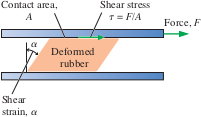
\includegraphics[width=8cm]{fig1}
\caption{Deformacion de una goma debido a una fuerza horizontal aplicada sobre la lamina superior \cite{this}.}
\label{f1}
\end{figure}


De la estatica de cuerpos podemos definir:
\begin{defn}
Estres se define como la fuerza por unidad de area y se calcula como fuerza $F$ divida por el area $A$ sobre la cual actua la fuerza. Al descomponer la fuerza actuante, la fuerza normal dividad por el area es el estres normal y la componente tangencial por unidad de area es el esfuerzo cortante. Por ejemplo en un fluido en reposo (esfuerzo cortante igual a cero), el esfuerzo normal es la presion.
\end{defn} 

Liquidos y gases (o vapores) se diferencian en que al tener un liquido en un contenedor, el volumen del liquido permanece constante formando una superficie libre porque la fuerza de cohesion entre las moleculas es alta y las moleculas estan cerca. En contraste, en un gas las moleculas se mueven aleatoriamente y estan mas alejadas y tienden a ocupar todo el volumen del contenedor debido a la debil fuerza cohesiva de sus moleculas (ver Figure~\ref{f2}). Fluidos como el asfalto o lodos se comportan como solidos y liquidos dependiente de la magnitud de los esfuerzos aplicados. 

\begin{figure}[h]
\centering
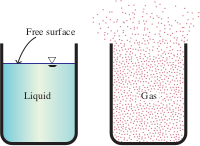
\includegraphics[width=8cm]{liqGas}
\caption{Liquidos y gases \cite{this}.}
\label{f2}
\end{figure}


\subsection{Clasificaci\'on de los fluidos}
\subsubsection{Flujos viscosos vs flujos inviscidos} 
La resistencia interna a fluir de un fluido es denominada como \textbf{viscosidad} el cual es una medida de la pegajosidad de un fluido. La viscosidad es causada por las fuerzas cohesivas entre moleculas en liquidos y por las coliciones molecurales en gases. Flujos en los cuales las fuerzas de fricci\'on son significantes son llamadas \textbf{flujos viscosos}. Sin embargo existen regiones en las cuales las fuerzas muy peque\~nas en comparacion con fuerzas inerciales y o de presion y son denominadas regiones de \textbf{flujo inviscido}.

\subsubsection{Flujos internos vs flujos externos} 
Un flujo es clasificado como externo o interno dependiendo de si fluye sobre una superficie o en un espacio confinado. Por ejemplo, el flujo sobre una lamina o un cilindro se deno\textbf{flujo externo}. El flujo a lo largo de una tuberia (e.g en un acueducto) se denomina \textbf{flujo interno}. En flujos internos son dominados por la viscosidad mientras que en flujos externos la viscosidad estan limitados a la capa limite.

\subsubsection{Flujos compresibles vs flujos incompresibles} 
Un \textbf{flujo compresible} es un flujo en el cual la densidad varia mientras un \textbf{flujo incompresible} es aquel en donde la densidad permanece constante (cada porcion del volumen del flujo permanece igual). Los liquidos son considerados como fluidos incompresibles mientras que los gases, los cuales cambian su densidad cuando son sometidos a presion, son considerados compresibles. Mientras que un fluido sometido a una presion igual 210 atm cambia su densidad en un 1\%, un gas cambia en la misma proporcion cuando se aumenta la presion en 0.01 atm. 


\subsubsection{Flujo laminar vs flujo turbulento}
Aquellos flujos que se mueven ordenadamente formando laminas de particulas que se mueven adyacentemente son denonominados \textbf{flujos laminares}. Flujos altamente viscosos como el aceite moviendose a velocidades bajas son tipicamente laminares. En contraste, flujos que mueven de manera desordenada debido a las altas velocidades son denominados \textbf{flujos turbulentos}. Flujos de baja viscosidad como el aire son considerados como turbulentos. Un flujo que cambia de laminar a turbulento o viceversa es un \textbf{flujo de transici\'on} (see Figura~\ref{fLamTur}). Los experimentos realizados por Osborne Reynolds en 1880 resultaron en el establecimiento del \textbf{Numero de Reynolds}, el cual es un numero adimensional que se usa para clasificar el regimen de flujo en tuberias.  

\begin{figure}[h]
\centering
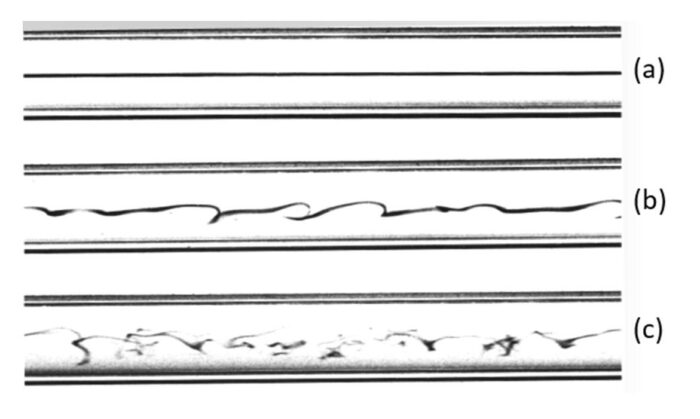
\includegraphics[width=8cm]{fLamTur}
\caption{a) flujo laminar, b) flujo de transicion y c) flujo turbulento (Ansys, Inc.).}
\label{fLamTur}
\end{figure}

\subsubsection{Flujos naturales vs flujos forzados}
Un flujo es natural o forzado dependiendo de como el movimiento del fluido es iniciado. Un \textbf{flujo forzado} es un  flujo cuyo movimento es iniciado por un medio externo como por ejemplo una bomba o un ventilador en una tuberia. En contraste, un \textbf{flujo natural} es produducido por medios naturales como por ejemplo el movimiento ascendente de flujos caliendes y el moviento descendiente de flujos frios en un lago gracias a los cambios de temperatura y por lo tanto de la densidad. 

\subsubsection{Flujo permanente vs flujo no permanente}
Un \textbf{flujo permanente} es aquel en donde propiedades como la velocidad, la temperature, etc en un punto no cambian en un intervalo de tiempo. Lo opuesto ocurre en \textbf{flujos no permanentes} o \textbf{flujos transitorios}. Bombas, compresores e intercanbiadores de calor funcionan, en terminos generales y por largos periodos de tiempo, bajo condiciones de flujo permanente a pesar que el flujo local se comporta como flujo no permanente. Esto quiere decir que la masa, el volumen y la energia tambien permanecen constantes. El estudio de flujos permanentes implica promediar caracteristicas de flujo como campos de flujo y de presi\'on (ver Figura~\ref{steNos}b). Sin embargo, si se requiere estudiar las vibraciones inducidades por un flujo, fluctuaciones de presion y ondas, es necesario consider el flujo como no permanente (ver Figura~\ref{steNos}a). 

\begin{figure}[h]
\centering
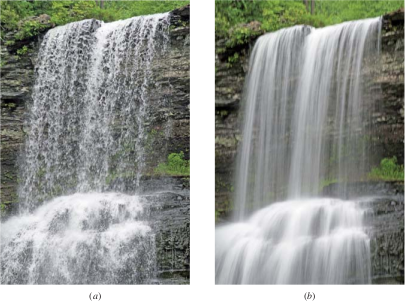
\includegraphics[width=8cm]{steNos}
\caption{a) foto instantanea de flujo (no permanente) y b) exposicion del flujo en un intervalo de tiempo \cite{this}.}
\label{steNos}
\end{figure}

\subsubsection{Flujo en una, dos y tres dimensiones}
Dependiendo de la distribuci\'on de la velocidad, un flujo puede ser clasificado como unidimensional, bidimensional o tredimensional. Un \textbf{flujo tredimensional (3D)} es aquel en el cual la velocidad cambia en las tres dimensiones espaciales; $\vec{V}(x,y,z)$ en coordenadas cartesianas o $\vec{V}(r,\theta,z)$ en coordenadas cilindricas. Cuando la variaci\'on de la velocidad es menor en cierta direcci\'on con respecto a otra direcci\'on, el flujo puede considerarse como \textbf{bidimensional (2D)} o \textbf{unidimensional (1D)}.
Consideremos un flujo permanente a travez de una tuberia circular conectada a un tanque (ver Figura~\ref{flowd}). De acuerdo a la condici\'on de no deslizamiento, la velocidad en las parededes de la tuberia es zero. El flujo es 2D en la regi\'on de entrada a la tuberia por que la velocidad cambia con respecto a la direcci\'on en $r$ y $z$. El perfil de velocidades en la tuberia al desarrollarse completamente despues de cierda distancia de la entrada se considera un flujo 1D por que solo varia en la direcci\'on radial $r$. Note que el flujo es 1D es coordenadas cilindricas y 2D en cordenadas cartersianas; de ah\'i la importancia de escoger correctamente el sistema de coordenadas. El flujo en rios peque\~nos puede considerarse como flujo 1D mientras que el flujo en lagos es usualmente considerado 3D.

\begin{figure}[h]
\centering
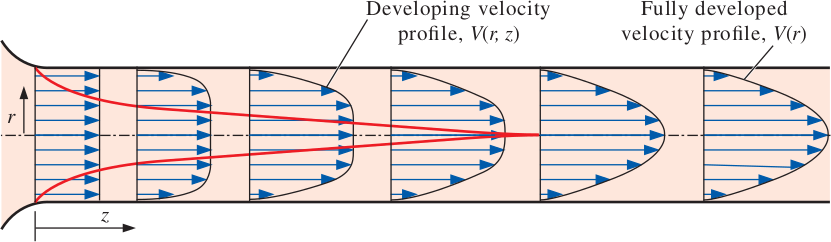
\includegraphics[width=8cm]{flowd}
\caption{Perfil de velocidad 2D, $\vec{V}(r,z)$, a la entrada de la tuberia. Este se convierte en 1D, $\vec{V}(r)$, a  cierta distancia de la entrada \cite{this}.}
\label{flowd}
\end{figure}


\subsection{Sistemas de unidades}
Cualquier cantidad es caracterizada por sus \textbf{dimensiones} y las magnitudes asignadas a las dimensiones son llamadas \textbf{unidades}.

\begin{defn}
\textbf{Dimensiones fundamentales} o \textbf{primaries} son la masa \{M\}, la longitud \{L\}, el tiempo \{T\} y la temperature \{$\Theta$\}. De estas se derivan por ejemplo las dimensiones de la velocidad $V$, de la energia $E$ y de el volumen $V$, estas son denominadas \textbf{dimensiones secundarias} o \textbf{dimensiones derivadas}.
\end{defn}

Existen dos sistemas de unidades: el \textbf{Sistema Ingles} y el \textbf{Sistema Internacional (SI)}. El SI esta basado relaciones decimales simples entre las unidades y es el mas usados (ver Tabla~\ref{t1}). El sistema Ingles relaciones abitraries entre unidades y es usado principalmente en Estados Unidos y el Reino Unido. 

\begin{table}[h!]
\centering
\begin{tabular}{l c}
 \hline
 Dimensi\'on & Unidad \\ [0.5ex]
 \hline\hline
 Longitud \{L\} & metro ($m$)  \\
 Masa \{M\} & kilogramo ($kg$)  \\
 Tiempo \{T\} & segundo ($s$)  \\
 Temperatura \{$\Theta$\} & kelvin ($K$)  \\
 Corriente el\'ectrica & amperio ($A$)  \\
 Intensidad de luz &  candela ($cd$) \\ 
 Cantidad de materia & mol ($mol$)  \\ [1ex]
 \hline
\end{tabular}
\caption{Las siete dimensiones fundamentales y sus unidades.}
\label{t1}
\end{table}

El SI esta basado en relaciones decimales entre unidades. Los prefijos usados para expresar los multiples de varios unidades estan en la Tabla~\ref{t2}. Estos prefijos son estandards para todas las unidades.

\begin{table}[h!]
\centering
\begin{tabular}{c c}
 \hline
 Multiplo & Prefijo \\ [0.5ex]
 \hline\hline
 10$^{24}$ & yotta, Y \\
 10$^{21}$ & zetta, Z \\
 10$^{18}$ & exa, E \\
 10$^{15}$ & peta, P \\
 10$^{12}$ & tera, T \\
 10$^{9}$ & giga, G \\
 10$^{6}$ & mega, M \\
 10$^{3}$ & kilo, k \\
 10$^{2}$ & hecto, h \\
 10$^{1}$ & deka, da \\
 10$^{-1}$ & deci, d \\
 10$^{-2}$ & centi, c \\
 10$^{-3}$ & mili, m \\
 10$^{-6}$ & micro, $\mu$ \\
 10$^{-9}$ & nano, n \\
 10$^{-12}$ & pico, p \\
 10$^{-15}$ & femto, f \\
 10$^{-18}$ & atto, a \\
 10$^{-21}$ & zepto, z \\
 10$^{-24}$ & yocto, y \\ [1ex]
  \hline
\end{tabular}
\caption{Prefijos estandard en el SI de unidades.}
\label{t1}
\end{table}


\subsubsection{Algunas unidades en SI y sistema Ingles}
En sistema Ingles, la masa, la longitud y el tiempo, estan dados en libras ($lbm$), pies ($ft$) y segundos ($s$). La equivalencia con el SI es:
$$
1 lb = 0.45359 kg
$$
$$
1 ft = 0.3048 m 
$$

Las unidades de fuerza son derivadas de la segunda ley de Newton:
$$
Fuerza = (masa) (aceleracion)
$$
$$
F = ma
$$
En SI las unidades de fuerza son newton $(N$), la cual es la fuerza requerida para acelerar una masa de 1 $kg$ a una rata de 1 $m s^{-2}$. En sistema Ingles las unidades de fueza son la libra fuerza ($lbf$) y es definida como la fuerza requerida para acelerar una masa de 1 $slug$ (32.174 $lbm$) a una rata de 1 $ft s^{-2}$. 

El peso de un objecto es la fuerza ejercida por la gravedad sobre dicho objeto y se detetermina aplicando la segunda ley de Newton, en donde $m$ es la masa del cuerpo y $a=g$ es la aceleraci\'on local de la gravedad g = 9.807 $m s^{-2}$ o g = 32.174 $ft s^{-2}$ a nivel del mar. $g$ cambia a grandes distancias de la tierra, pero puede considerarse constante para el analisis fisico de objetos terrestres. La masa es la misma en cualquier parte del universo. Utilizando el concepto de peso, 1 $N$ es equivalente al peso de ~1 manzana (m = 102 $g$); 1 $lbf$ equivalente al peso de ~4 manzanas (m = 454 g). El peso por unidad de volume es llamado peso espefifico $\gamma = \rho g$ donde $rho$ es la densidad. 

El \textbf{trabajo} el cual es una forma de energia se define como el producto entre fuerza y distancia y sus unidades es el  joule ($J$):
$$
1J = 1 N.m
$$

1 caloria ($cal$) es definidad como la cantidad de trabajo necesario para incrementar en 1 $^oC$ la temperatura de un gramo de agua a una temperatura de 14.5 $^oC$. La \textbf{potencia} es conocidada como el trabajo por unidad de tiempo y esta dada en watt ($W$ = $J s^{-1}$). Otra unidad conocida son los caballos de potencia; $1 hp = 745.7 W$. La energia electrica es tipicamente expresada en kilowatt-hora $kWh$ equivalente a 3600 $kJ$. Por ejemplo, un electrodomestico con una potencia de 1 $kW$ consume 1 $1kWh$ de electricidad funcionando continuamente durante una hora.


\subsubsection{Dimensiones homogeneas y conversi\'on de unidades}
En ingenieria y ciencias, todas las ecuaciones deben ser dimensionalmente homogeneas, esto quiere decir que las cantidades que se suman o restan en la equacion tienen las mismas dimensiones. Por ejemplo, en la ecuaci\'on de Bernoulli para flujo incompresible:
$$
p + \frac{1}{2} \rho V^2 + \rho g Z = constante
$$
todos los terminos de la ecuaci\'on tienen dimensiones de presi\'on $[ML^{-1}T^{-2}]$.

Como lo habiamos expresado antes, las unidades secundarias son aquellas que se expresan con base en unidades primarias. Por ejemplo, la fuerza esta expresada como:
$$
N=kg\frac{m}{s^2}
$$
$$
lbf = 32.174 \text{ lbm$\frac{ft}{s^2}$}
$$

Estas pueden expresarse como \textbf{fracciones de conversion unitarias}:
$$
\frac{N}{kg.m/s^2} = 1
$$
$$
\frac{lbf}{32.174lbm.ft/s^{2}} = 1
$$
y son \'utiles para la conversi\'on de unidades.

\begin{shaded}
\begin{exa}
Un cuerpo pesa 1000 lbf en la tierra donde la gravedad es g = 32.174 ft s$^{-2}$. a) ¿Cual es la masa en kg? b) ¿Cual es el peso de este cuerpo en N en la luna donde la gravedad es g$_{moon}$ = 1.62 m s$^{-2}$? c) ¿Que tan rapido el cuerpo es acelerado si la fuerza neta aplicada sobre este 400 lbf en la tierra o en la luna?
\vspace{0.2cm}
\hrule
\vspace{0.2cm}
\noindent \textbf{Soluci\'on}
\vspace{0.2cm}
\hrule
\vspace{0.2cm}
\noindent \textbf{Parte a}\\ 
De acuerdo con la ley de Newton:
$$
F=W=1000 \text{ lbf} = mg=(m)(32.174 \text{ ft/s$^2$})
$$
despejando para $m$, tenemos:
$$
m = \frac{1000 \text{ lbf}}{32.174 \text{ ft/s$^2$}} = 31.08 \text{ slugs}
$$
convirtiendo a kg:
$$
m = 31.08 \text{ slugs} = (31.08 \text{ slugs})(14.5939 \text{ kg/slugs}) = 454 \text{ kg}
$$
\begin{center}
\textcolor{red}{\textbf{La masa del cuerpo es 454 kg}}
\end{center}

\noindent \textbf{Parte b}\\
Teniendo en cuenta que la masa calculada igua a 454 kg es la misma en cualquier parte del universo, usando la segunda ley de Newton:
$$
F = W_{luna} = mg_{luna} = (454\text{ kg})(1.62 \text{ m/s$^2$})=735 \text{ N}
$$
\begin{center}
\textcolor{red}{\textbf{El peso del cuerpo en la luna es 735 N}}
\end{center}

\noindent \textbf{Parte c}\\
Aplicando la segunda ley de Newton y teniendo en cuenta que la masa permanece constante:
$$
F = 400 \text{ lbf} = ma = (31.08 slugs)a
$$
despejando a:
$$
a = \frac{400 \text{ lbf}}{31.08 \text{ slugs}} = 12.87 \text{ $\frac{ft}{s^2}$} \left( 0.3048\text{ $\frac{m}{ft}$} \right) = 3.92 \text{ m/s$^2$}
$$

\begin{center}
\textcolor{red}{\textbf{La aceleraci\'on del cuerpo sometido a dicha fuerza en cualquier parte es 3.92 m s$^{-2}$}}
\end{center}

\end{exa}
\end{shaded}



\begin{shaded}
\begin{exa}
La formula de Stokes-Oseen 
$$
F=3\pi \mu D V + \frac{9 \pi}{16} \rho V^2 D^2
$$
sirve para calcular la fuerza de arrastre F de una esfera de diametro D en un fluido a velocidad baja V, con un densidad $\rho$ y con una viscosidad $\mu$. ¿Es la formula dimensionalmente homogenea?
\vspace{0.2cm}
\hrule
\vspace{0.2cm}
\noindent \textbf{Soluci\'on}
\vspace{0.2cm}
\hrule
\vspace{0.2cm}

De la segunda ley de Newton, $F=ma$,  cuyas unidades son $\{M\} \{L T^{-2}\}$. Renplazando las unidades en la equaci\'on:
$$
\{M\} \{L T^{-2}\} = 3\pi \{M L^{-1} T^{-1}\} \{L\} \{L T^{-1}\} + \frac{9\pi}{16} \{M L^{-3}\} \{L^2 T^{-2}\} \{L^2\} 
$$

simplificando el lado izquierdo de la equaci\'on:

$$
\{M\} \{L T^{-2}\} = 3\pi \{M L T^{-2}\} + \frac{9\pi}{16}  \{M L T^{-2}\}
$$

\begin{center}
\textcolor{red}{\textbf{La equaci\'on de Stokes-Oseen es dimensionalmente homogenea.}}
\end{center}

\end{exa}
\end{shaded}



\begin{shaded}
\begin{exa}
La figure muestra el flujo sobre una presa. El caudal Q es conocido y depende del ancho de la cresta de la presa B, la aceleracion de la gravedad g, y de la profundidad aguas arriba por encima de la cresta. Es conocido que Q es proporcional a B. ¿Como es la equaci\'on para estimar Q?       
\begin{center}
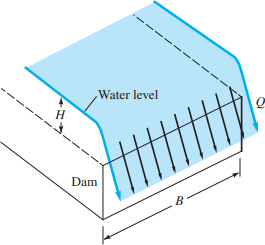
\includegraphics[width=4cm]{pdam}
\end{center}
\vspace{0.2cm}
\hrule
\vspace{0.2cm}
\noindent \textbf{Soluci\'on}
\vspace{0.2cm}
\hrule
\vspace{0.2cm}
De acuerdo con el problema sabemos que $Q=f(B,g,H)$ y que $Q\propto B$. Las unidades de las variables son:
$$
Q\ \frac{\{L^3\}}{\{T\}}; \quad B \ \{L\}; \quad g \ \frac{\{L\}}{\{T^2\}}; \quad H \ \{L\}
$$

Teniendo en cuenta que la funci\'on $Q=f(B,g,H)$ deber ser dimensionalmente homogenea; ambos lados de la ecuacio\'on deben tener las mimas unidades, tenemos que: 

$$
\frac{\{L^3\}}{\{T\}} \propto \{L\}  \frac{\{L\}^{1/2}}{\{T^2\}^{1/2}} \{L^{3/2}\}
$$

simplificando:

$$
\frac{\{L^3\}}{\{T\}} \propto \frac{\{L^3\}}{\{T\}}
$$


\begin{center}
\textcolor{red}{\textbf{La funcion para Q es $Q = C \ B \ g^{1/2} \ H^{3/2}$ donde C es una constante de proporcionalidad.}}
\end{center}





\end{exa}
\end{shaded}





%\subsection{Fri, Sept 6: Phenomenology of Microscopic Physics}
%
%\begin{itemize}
%
%\item Newtonian mechanics (i.e., ${\bf F} = m{\bf a}$) is an excellent theory; it applies to the vast majority of human-scale (and even interplanetary-scale) physics. 
%
%\item Apart from relativistic effects at very high velocities (special relativity) or in very strong gravitational fields (general relativity), Newtonian mechanics accurately describes a huge range of phenomena, but around the end of the Nineteenth Century people became aware of some physical effects for which there is no sensible Newtonian explanation.
%
%\item Examples include:
%\begin{itemize}
%\item the {\bf double slit experiment} (done with light by Thomas Young in 1801, and with electrons by Tonomura in 1986)
%\item the photoelectric effect (analyzed by Einstein in 1905 --- in fact his Nobel-winning work)
%\item the ``quantum Venn diagram'' puzzle, involving the overlaps of three polarizing filters
%\item the stability of the hydrogen atom (i.e., the fact that the electron doesn't lose energy and spiral inward toward the proton).
%\end{itemize}
%
%\begin{rem}
%How now, brown cow?
%\end{rem}
%
%\begin{defn}
%The {\em Feynman kernel} is given by
%\[ K(x_b, t_b; x_a, t_a) = \int_{x(t_a) = x_a}^{x(t_b) = x_b} e^{(i/\hbar) S[x(t)]} \; \mathcal{D}x(t). \]
%\end{defn}
%
%\end{itemize}
%
%\subsection{Mon, Sept 9: Review of Newtonian Mechanics}
%
%\begin{itemize}
%
%\item  A {\em Newtonian trajectory} ${\bf x}(t)$ ($t \in \R$) is given by solutions of the second order ODE
%\[ m\, \ddot{{\bf x}}(t) = {\bf F}({\bf x}(t)), \]
%where $m > 0$ is a basic parameter associated with a given Newtonian particle, called its {\em mass}.
%
%\item The force field ${\bf F}({\bf x})$ --- which we take to be static (i.e., not intrinsically dependent on time) for simplicity --- is said to be {\em conservative} if there is a {\em potential function} $V({\bf x})$ such that
%\[ {\bf F}({\bf x}) = -\nabla V({\bf x}). \]
%Here, `$\nabla$' denotes the {\em gradient operator}, 
%\[ \nabla V = \bigg( \frac{\partial V}{\partial x}, \, \frac{\partial V}{\partial y}, \, \frac{\partial V}{\partial z} \bigg). \]
%
%\item For a conservative force field, we can find a {\em conserved quantity} along the Newtonian trajectories, namely the {\em total mechanical energy}.
%\[ E = H({\bf x}, {\bf p}) := \frac{1}{2m}\, {\bf p}^2 + V({\bf x}). \]
%Here, ${\bf p}^2 := {\bf p} \Cdot {\bf p} = \| {\bf p} \|^2$, and ${\bf p} := m {\bf v} := m \dot{{\bf x}}$ is the {\em momentum}.
%
%\end{itemize}
%
%\subsection{Tue, Sept 10: Alternative Formulations of Newtonian Mechanics}
%
%\begin{itemize}
%
%\item The {\bf Hamiltonian formulation}:
%\[ \dot{{\bf x}} = \frac{\partial H}{\partial {\bf p}}, \;\;\;\;\; \dot{{\bf p}} = - \frac{\partial H}{\partial {\bf x}}. \]
%
%\item The {\bf Lagrangian formulation}:
%\[ \delta S[{\bf x}(t)] = 0, \]
%where the {\em action} on the time interval $[t_a, t_b]$ is given by
%\[ S[{\bf x}(t)] := \int_{t_a}^{t_b} \bigg[ \frac{m}{2} \, \dot{{\bf x}}(t)^2 - V({\bf x}(t)) \bigg]  \; dt. \]
%
%\item Etc.
%
%\end{itemize}
%
%
%\section{Spring 2020}



\end{document}
